%%%%%%%%%%%%%%%%%%%%%%%%%%%%%%%%%%%%%%%%%%%%%%%%%%%%%%%%%%%%%%%%%%%%%%%%%%%%%%%%
% Template for USENIX papers.
%
% History:
%
% - TEMPLATE for Usenix papers, specifically to meet requirements of
%   USENIX '05. originally a template for producing IEEE-format
%   articles using LaTeX. written by Matthew Ward, CS Department,
%   Worcester Polytechnic Institute. adapted by David Beazley for his
%   excellent SWIG paper in Proceedings, Tcl 96. turned into a
%   smartass generic template by De Clarke, with thanks to both the
%   above pioneers. Use at your own risk. Complaints to /dev/null.
%   Make it two column with no page numbering, default is 10 point.
%
% - Munged by Fred Douglis <douglis@research.att.com> 10/97 to
%   separate the .sty file from the LaTeX source template, so that
%   people can more easily include the .sty file into an existing
%   document. Also changed to more closely follow the style guidelines
%   as represented by the Word sample file.
%
% - Note that since 2010, USENIX does not require endnotes. If you
%   want foot of page notes, don't include the endnotes package in the
%   usepackage command, below.
% - This version uses the latex2e styles, not the very ancient 2.09
%   stuff.
%
% - Updated July 2018: Text block size changed from 6.5" to 7"
%
% - Updated Dec 2018 for ATC'19:
%
%   * Revised text to pass HotCRP's auto-formatting check, with
%     hotcrp.settings.submission_form.body_font_size=10pt, and
%     hotcrp.settings.submission_form.line_height=12pt
%
%   * Switched from \endnote-s to \footnote-s to match Usenix's policy.
%
%   * \section* => \begin{abstract} ... \end{abstract}
%
%   * Make template self-contained in terms of bibtex entires, to allow
%     this file to be compiled. (And changing refs style to 'plain'.)
%
%   * Make template self-contained in terms of figures, to
%     allow this file to be compiled. 
%
%   * Added packages for hyperref, embedding fonts, and improving
%     appearance.
%   
%   * Removed outdated text.
%
%%%%%%%%%%%%%%%%%%%%%%%%%%%%%%%%%%%%%%%%%%%%%%%%%%%%%%%%%%%%%%%%%%%%%%%%%%%%%%%%

\documentclass[letterpaper,twocolumn,10pt]{article}
\usepackage{usenix2019_v3}

% to be able to draw some self-contained figs
\usepackage{tikz}
\usepackage{amsmath}

% inlined bib file
\usepackage{filecontents}

%-------------------------------------------------------------------------------
%\begin{filecontents} \include{\jobname.bib}
%\end{filecontents}

%-------------------------------------------------------------------------------
\begin{document}
%-------------------------------------------------------------------------------

%don't want date printed
\date{}

% make title bold and 14 pt font (Latex default is non-bold, 16 pt)
\title{\Large \bf Submission}

%for single author (just remove % characters)
\author{
{\rm Anon}\\
DoubleBlind
% copy the following lines to add more authors
% \and
% {\rm Name}\\
%Name Institution
} % end author

\maketitle

%-------------------------------------------------------------------------------
\begin{abstract}
%-------------------------------------------------------------------------------
Your abstract text goes here. Just a few facts. Whet our appetites.
Not more than 200 words, if possible, and preferably closer to 150.
\end{abstract}


%-------------------------------------------------------------------------------
\section{Introduction}
%-------------------------------------------------------------------------------
Strongly consistent distributed databases (DSDBs) provide scalable storage capacities for large scale web applications without sacrificing easy-to-reason-about concurrency semantics. However, they do not achieve good throughput under skewed workloads, even though real-world workloads are inherently skewed. On the other hand, single machine databases (SMDBs) better accommodate skew in their workloads due to their throughputs being higher by several orders of magnitude. In exchange, their storage capacities cannot scale past a single machine.

When searching for a database to support skewed workloads, users are forced to choose between performant SMDBs or scalable DSDBs. Skew creates “hotkeys” which are highly contended for. In a distributed setting, hotkeys are a product of uneven load concentrated on a few keys that ultimately leave some nodes overwhelmed but others underutilized. In addition, contention induces cycles of deadlocks, wait queues, retries, and aborts that the database from efficiently utilizing nodes’ processing power to execute transactions.

A DSDB’s throughput can easily scale with the number of nodes in the case of uniform or partitionable workloads via load balancing techniques like sharding, but these techniques are poorly suited for the case of highly skewed workloads. Hotkeys inundate their host nodes (“hotshards”) beyond their maximum throughputs such that requests cannot be processed fast enough to clear a growing queue. The hotshards cannot clear their large workload fast enough because they are not sufficiently provisioned--either in terms of hardware or software--to sustain such high throughput. Without provisioning very powerful hotshards, the hotshards themselves become a bottleneck for system throughput.

SMDBs accommodate skewed workloads better than their distributed counterparts because they sustain fundamentally higher throughput. The primary reason for this is that SMDBs need not communicate over a network. While an RPC between two nodes in the same datacenter costs at least a few milliseconds, a message between two CPU cores costs at most a few microseconds. Thus, distributed transactions take several orders of magnitude longer to complete. The communication cost decreases throughput by decreasing the number of transactions that the database can eke out per unit time simply because transactions have a higher latency. A DSDB’s communication cost is a fundamental bottleneck that prevents it from achieving the same throughput as SMDBs.

Furthermore, the high latency of distributed transactions generates more contention on popular keys at lower skews. Contention is a serious bottleneck in strongly consistent systems that prevents systems from utilizing their nodes’ throughput capability for executing transactions; no useful work is done when transactions expend node resources waiting, retrying, or aborting instead of committing. These systems often implement concurrency control protocols such as 2PL or OCC that lock keys for significant durations of time, making them more prone to contention than their weakly consistent counterparts. Skew induces contention, because it creates a small set of hotkeys that a large proportion of requests will attempt to lock. Only one transaction can lock any given key at a time, so high contention forces transactions to serialize their execution on hotkeys. This effectively reduces the system’s throughput to the processing rates of individual nodes. In a distributed setting, transactions’ higher latencies prolong the durations for which the transactions hold locks, exacerbating the conflict. At best, this results in head-of-line blocking. More likely, following transactions that fail to acquire their locks will repeatedly retry, deadlock, and/or abort, all of which leads to decreased system throughput.

We introduce Thermopylae, a distributed database that offers throughput on the order of magnitude of a SMDB. Thermopylae introduces a novel architecture that embeds a SMDB into a DSDB. We exploit the inherent skew in real world workloads and co-locate hotkeys on a single hotshard to create a central point to which we can apply targeted optimizations. We then completely replace the hotshard with a SMDB instance, which we fully integrate into the overall DSDB. The novel architecture and co-location together prevent the hotshard from becoming a bottleneck by applying the SMDB’s superior throughput to the workload’s hottest keys. In order to alleviate contention and enable Thermopylae to access the full throughput capability of our novel architecture, we design a complementary concurrency control protocol, 3PL, that reduces contention on the hotshard and coordinates two distinctly executing databases to preserve strict serializability. 

\rewrite{\textbf{<Here is a paragraph reserved for eval numbers.>} Lorem ipsum lorem ipsum text text text.}

In summary, this paper makes the following contributions:
\begin{itemize}
    \item A novel distributed architecture that increases throughput \true{by several orders of magnitude}.
    \item An complementary concurrency control protocol that enforces strict serializability by coordinating two independent databases.
    \item \true {Thermopylae, a distributed database capable of sustaining throughput around three orders of magnitude higher than existing state of the art.}
\end{itemize}
\section{Background}
\jenndebug{need some filler here.}



\subsection{Transactions}

\subsection{Single Machine Databases}
\rewrite{\textbf{Paragraph's purpose: what are they? Just a single sentence should do.}}

\rewrite{\textbf{Paragraph (or two)'s purpose: why SMDBs offer good performance.}}
\cite{ermia, cicada, silo, mocc}

\subsection{Distributed Databases}
\rewrite{\textbf{Paragraph's purpose: what are they? What need were they initially trying to fill that SMDBs could not?}}

\rewrite{\textbf{Paragraph (or two)'s purpose: why are they so bad at performance?}}

\rewrite{\textbf{Paragraph's purpose: list the use case under which distributed databases work really well aka partitionable workloads in which all partitions receive roughly equal load.}}

\subsection{Skew}
\rewrite{\textbf{Paragraph's purpose: what is skew? Garlic graph?}}

\rewrite{\textbf{Paragraph's purpose: what workloads are illustrative of what skews?}}

\rewrite{\textbf{How do we use exploit skew in our database?}}

%-------------------------------------------------------------------------------
\section{Footnotes, Verbatim, and Citations}
%-------------------------------------------------------------------------------

Footnotes should be places after punctuation characters, without any
spaces between said characters and footnotes, like so.%
\footnote{Remember that USENIX format stopped using endnotes and is
  now using regular footnotes.} And some embedded literal code may
look as follows.

\begin{verbatim}
int main(int argc, char *argv[]) 
{
    return 0;
}
\end{verbatim}

Now we're going to cite somebody. Watch for the cite tag. Here it
comes. Arpachi-Dusseau and Arpachi-Dusseau co-authored an excellent OS
book, which is also really funny~\cite{fblinchpin}, and
Waldspurger got into the SIGOPS hall-of-fame due to his seminal paper
about resource management in the ESX hypervisor~\cite{fbphotocaching}.

The tilde character (\~{}) in the tex source means a non-breaking
space. This way, your reference will always be attached to the word
that preceded it, instead of going to the next line.

And the 'cite' package sorts your citations by their numerical order
of the corresponding references at the end of the paper, ridding you
from the need to notice that, e.g, ``Waldspurger'' appears after
``Arpachi-Dusseau'' when sorting references
alphabetically~\cite{fblinchpin, fbphotocaching}. 

It'd be nice and thoughtful of you to include a suitable link in each
and every bibtex entry that you use in your submission, to allow
reviewers (and other readers) to easily get to the cited work, as is
done in all entries found in the References section of this document.

Now we're going take a look at Section~\ref{sec:figs}, but not before
observing that refs to sections and citations and such are colored and
clickable in the PDF because of the packages we've included.

%-------------------------------------------------------------------------------
\section{Floating Figures and Lists}
\label{sec:figs}
%-------------------------------------------------------------------------------


%---------------------------
\begin{figure}
\begin{center}
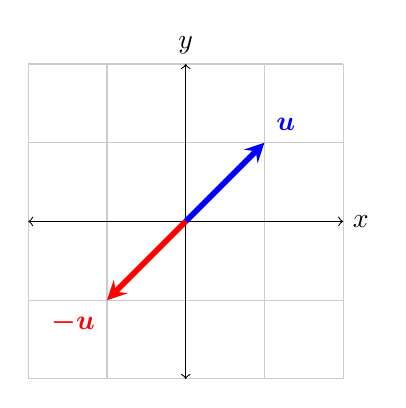
\begin{tikzpicture}
  \draw[thin,gray!40] (-2,-2) grid (2,2);
  \draw[<->] (-2,0)--(2,0) node[right]{$x$};
  \draw[<->] (0,-2)--(0,2) node[above]{$y$};
  \draw[line width=2pt,blue,-stealth](0,0)--(1,1)
        node[anchor=south west]{$\boldsymbol{u}$};
  \draw[line width=2pt,red,-stealth](0,0)--(-1,-1)
        node[anchor=north east]{$\boldsymbol{-u}$};
\end{tikzpicture}
\end{center}
\caption{\label{fig:vectors} Text size inside figure should be as big as
  caption's text. Text size inside figure should be as big as
  caption's text. Text size inside figure should be as big as
  caption's text. Text size inside figure should be as big as
  caption's text. Text size inside figure should be as big as
  caption's text. }
\end{figure}
%% %---------------------------


Here's a typical reference to a floating figure:
Figure~\ref{fig:vectors}. Floats should usually be placed where latex
wants then. Figure\ref{fig:vectors} is centered, and has a caption
that instructs you to make sure that the size of the text within the
figures that you use is as big as (or bigger than) the size of the
text in the caption of the figures. Please do. Really.

In our case, we've explicitly drawn the figure inlined in latex, to
allow this tex file to cleanly compile. But usually, your figures will
reside in some file.pdf, and you'd include them in your document
with, say, \textbackslash{}includegraphics.

Lists are sometimes quite handy. If you want to itemize things, feel
free:

\begin{description}
  
\item[fread] a function that reads from a \texttt{stream} into the
  array \texttt{ptr} at most \texttt{nobj} objects of size
  \texttt{size}, returning returns the number of objects read.

\item[Fred] a person's name, e.g., there once was a dude named Fred
  who separated usenix.sty from this file to allow for easy
  inclusion.
\end{description}

\noindent
The noindent at the start of this paragraph in its tex version makes
it clear that it's a continuation of the preceding paragraph, as
opposed to a new paragraph in its own right.


\subsection{LaTeX-ing Your TeX File}
%-----------------------------------

People often use \texttt{pdflatex} these days for creating pdf-s from
tex files via the shell. And \texttt{bibtex}, of course. Works for us.

%-------------------------------------------------------------------------------
\section*{Acknowledgments}
%-------------------------------------------------------------------------------

The USENIX latex style is old and very tired, which is why
there's no \textbackslash{}acks command for you to use when
acknowledging. Sorry.

%-------------------------------------------------------------------------------
\section*{Availability}
%-------------------------------------------------------------------------------

USENIX program committees give extra points to submissions that are
backed by artifacts that are publicly available. If you made your code
or data available, it's worth mentioning this fact in a dedicated
section.

%-------------------------------------------------------------------------------
\bibliographystyle{plain}
\bibliography{jobname.bib}

%%%%%%%%%%%%%%%%%%%%%%%%%%%%%%%%%%%%%%%%%%%%%%%%%%%%%%%%%%%%%%%%%%%%%%%%%%%%%%%%
\end{document}
%%%%%%%%%%%%%%%%%%%%%%%%%%%%%%%%%%%%%%%%%%%%%%%%%%%%%%%%%%%%%%%%%%%%%%%%%%%%%%%%

%%  LocalWords:  endnotes includegraphics fread ptr nobj noindent
%%  LocalWords:  pdflatex acks